\documentclass[10pt]{article}

\usepackage[letterpaper,margin=0.85in]{geometry}
\usepackage{amsmath,amssymb}
\usepackage{graphicx}
\usepackage{booktabs}
\usepackage{array}
\usepackage{url}
\usepackage[colorlinks=true,linkcolor=black,citecolor=black,urlcolor=black]{hyperref}
\usepackage{placeins}

\graphicspath{{../../}{../../results/}{../}{../onboard/figures/}{figures/}}
\setlength{\parindent}{1em}
\renewcommand{\arraystretch}{1.08}
\emergencystretch=2em

\newcommand{\vect}[1]{\mathbf{#1}}
\newcommand{\mat}[1]{\mathbf{#1}}
\newcommand{\unit}[1]{\hat{\mathbf{#1}}}
\newcommand{\LU}{\mathrm{LU}}
\newcommand{\TU}{\mathrm{TU}}
\newcommand{\ND}{\mathrm{ND}}
\newcommand{\chisq}{\chi^2}

\title{\vspace{-0.35in}Supplemental Material:\\
Guidance-Coupled Bearing-Only Optical Navigation for Cislunar Transfers}
\author{Varsha Krishnakumar}
\date{May 2026}

\begin{document}
\maketitle

This supplement carries the extended sweeps and detailed sensitivity studies summarized in Section~5.7 of the main paper.  All experiments are $n=1000$ matched-seed Monte Carlo at the canonical operating point ($\sigma_{\rm px}=1$ pixel, $q_a=10^{-14}$, $t_c=2.0$, estimate-driven active pointing, $\vect{P}_0=\mathrm{diag}(10^{-6}\mat{I}_3,10^{-7}\mat{I}_3)$) unless explicitly varied.  Section-numbering uses an ``S'' prefix for clarity.  Every figure/table here has a backing $n=1000$ production CSV under \texttt{paper\_artifacts/} or \texttt{results/mc/} in the project repository; the figure-to-script manifest is \texttt{docs/experiment\_manifest.md}.

\section{Process-Noise Tuning}
\label{sec:S-qacc}
The process-noise study was performed in two stages.  A coarse sweep exposed the failure mode: too little process noise made the filter overconfident, with NEES far above the $\chisq(6)$ range.  A later fine sweep ran $1000$ trials at each of $11$ candidate $q_a$ values in the final operating regime.  Table~\ref{tab:S-qacc} shows that $q_a=10^{-9}$ would put the trial-mean NEES inside the diagnostic $\chisq(6)$ $95\%$ band on $99.4\%$ of trials but inflate the median terminal miss to $1.81\times10^{-4}\,\LU\approx 70.6$~km, while the lowest $q_a$ values preserve the $99.1\%$ screening pass rate at the price of a $89\%$ NEES band fraction.  The main paper adopts $q_a=10^{-14}$ as the canonical operating point so the realism sweeps (Sections~\ref{sec:S-attitude}--\ref{sec:S-delay}) operate inside the same covariance regime.

\begin{table}[h]
\centering
\caption{Fine process-noise sweep, $1000$ trials per point.  ``Band'' is the fraction of trial-mean NEES values inside the $\chisq(6)$ 95\% interval.}
\label{tab:S-qacc}
\footnotesize
\begin{tabular}{@{}lcccc@{}}
\toprule
$q_a$ & Pass & Miss med.\ [LU] & NEES med. & Band \\
\midrule
$1.0\times10^{-12}$  & 0.991 & $1.58\times10^{-4}$ & 5.77 & 0.893 \\
$3.16\times10^{-12}$ & 0.991 & $1.57\times10^{-4}$ & 5.74 & 0.899 \\
$1.0\times10^{-11}$  & 0.991 & $1.58\times10^{-4}$ & 5.71 & 0.905 \\
$3.16\times10^{-11}$ & 0.991 & $1.58\times10^{-4}$ & 5.57 & 0.925 \\
$1.0\times10^{-10}$  & 0.991 & $1.57\times10^{-4}$ & 5.22 & 0.944 \\
$3.16\times10^{-10}$ & 0.991 & $1.67\times10^{-4}$ & 4.82 & 0.977 \\
$1.0\times10^{-9}$   & 0.991 & $1.81\times10^{-4}$ & 4.34 & 0.994 \\
$3.16\times10^{-9}$  & 0.989 & $2.33\times10^{-4}$ & 3.92 & 0.998 \\
$1.0\times10^{-8}$   & 0.970 & $2.90\times10^{-4}$ & 3.62 & 0.996 \\
$3.16\times10^{-8}$  & 0.942 & $3.37\times10^{-4}$ & 3.30 & 0.995 \\
$1.0\times10^{-7}$   & 0.904 & $3.75\times10^{-4}$ & 2.97 & 0.995 \\
\bottomrule
\end{tabular}
\end{table}

\section{Sensitivity Studies (legacy $n=80$)}
The pixel-noise and $t_c$ sensitivity uses an earlier $n=80$ deterministic-seed configuration with active pointing and $q_a=10^{-9}$.  Pixel noise is manageable through $\sigma_{\rm px}=3$: the median terminal miss stays below the $10^{-3}\,\LU$ tolerance, rising from $1.22\times10^{-4}\,\LU$ at $\sigma_{\rm px}=0.5$ to $6.95\times10^{-4}\,\LU$ at $\sigma_{\rm px}=3$.  At $\sigma_{\rm px}=5$ the median reaches $1.73\times10^{-3}\,\LU$ and the upper tail is well outside tolerance.  Correction time shows a separate geometric effect: at $\sigma_{\rm px}=1.5$ the median miss drops from $1.32\times10^{-3}\,\LU$ at $t_c=0.8$ to $1.55\times10^{-4}\,\LU$ at $t_c=3.0$.

\section{Attitude Uncertainty}
\label{sec:S-attitude}
The baseline assumes ideal pointing.  Zero-mean rotational noise $\vect{\theta}\sim\mathcal{N}(\vect{0},\sigma_{\rm att}^2\mat{I}_3)$ is applied to the camera attitude at every measurement step on the truth side only; the filter back-projects through the unperturbed commanded DCM.  Sweeping $\sigma_{\rm att}\in\{0,0.001,0.003,0.01,0.03,0.1,0.3,1.0\}$ degrees at $n=1000$ yields the graceful-degradation curve in Table~\ref{tab:S-attitude}.  The median terminal miss is statistically indistinguishable from the no-noise baseline through $\sigma_{\rm att}=0.03^{\circ}$ ($61.6$--$64.5$ km), inflates to $88$~km at $0.1^{\circ}$, and then climbs steeply to $231$~km at $0.3^{\circ}$ and $1058$~km at $1^{\circ}$.

\begin{table}[h]
\centering
\caption{Attitude-noise sweep, $n=1000$ trials per $\sigma_{\rm att}$.}
\label{tab:S-attitude}
\footnotesize
\begin{tabular}{@{}cccccc@{}}
\toprule
$\sigma_{\rm att}$ [deg] & $n$ & miss med [km] & miss p95 [km] & NIS med. & NEES band \\
\midrule
0.000 & 1000 &   61.64 &  228.27 &  1.94 & 0.893 \\
0.001 & 1000 &   63.34 &  233.80 &  1.95 & 0.910 \\
0.003 & 1000 &   63.75 &  231.42 &  1.95 & 0.909 \\
0.010 & 1000 &   63.21 &  232.57 &  1.96 & 0.902 \\
0.030 & 1000 &   64.49 &  244.20 &  2.04 & 0.893 \\
0.100 & 1000 &   88.01 &  321.89 &  2.89 & 0.760 \\
0.300 & 1000 &  231.04 &  836.06 & 10.50 & 0.019 \\
1.000 & 1000 & 1057.99 & 3158.46 & 97.88 & 0.000 \\
\bottomrule
\end{tabular}
\end{table}

\begin{figure}[h]
\centering
\includegraphics[width=0.9\linewidth]{../../results/mc/phase_e_attitude_noise/06q_attitude_noise_sweep.png}
\caption{Attitude-noise sensitivity, $n=1000$ per $\sigma_{\rm att}$ point.  Median and 95th-percentile terminal miss on the left; median Moon-center NIS and median NEES on the right.  The performance plateau extends to roughly $0.1^{\circ}$ before the filter becomes inconsistent and miss climbs steeply.}
\label{fig:S-attitude}
\end{figure}

\section{Cumulative-Parallax Range Observability}
A bearing-only filter cannot observe range directly.  Range becomes observable through the cumulative angular change of the Moon line-of-sight relative to the trajectory.  Sweeping $t_c\in\{0.25,0.5,1.0,1.5,2.0,3.0,4.0,5.0\}$ at $n=1000$ trials per $t_c$ yields one (parallax, range error) point per trial.  The fit recovers an exponent of $-0.57$ against cumulative parallax (and $-0.71$ against the endpoint-to-endpoint quantity); both exponents are negative and order-unity, consistent with the bearing-only intuition that range error decays with accumulated LOS sweep but weaker than a clean inverse law because (a) very-short-arc bins are pre-convergence and (b) long-arc bins flatten at the noise floor.

\begin{figure}[h]
\centering
\includegraphics[width=0.9\linewidth]{../../results/mc/phase_e_parallax/06m_parallax_vs_range.png}
\caption{Cumulative-parallax versus range-error fit, $n=8000$ trials.  Empirical exponent $-0.57$.}
\label{fig:S-parallax}
\end{figure}

\section{Filter-Covariance Geometry at Burn}
The IEKF position covariance at $t_c$ is anisotropic: the elongated direction aligns with the weak observability mode reported in Section~4 of the main paper.  Whether that elongated direction matters for guidance depends on its alignment with the burn sensitivity, captured by the position-to-velocity STM block $\Phi_{rv}(t_f,t_c)$.

\begin{figure}[h]
\centering
\includegraphics[width=0.9\linewidth]{../../results/mc/phase_e_covariance/06j_covariance_ellipses_seed7.png}
\caption{$1\sigma$ and $3\sigma$ IEKF position-covariance ellipses at the burn epoch $t_c$ in three orthogonal planes, with the realized truth residual overlaid.}
\label{fig:S-covariance}
\end{figure}

\section{Initial-Covariance Robustness}
The $\vect{P}_0$ scale is swept by factors $\{1,3,10,30,100\}$ at $n=1000$ trials each.  Median miss inflates from $61.6$~km at the baseline scale to $116.4$~km at $\vect{P}_0\times 100$ (less than $2\times$ degradation across two orders of magnitude in initial covariance), and NIS stays essentially flat at $1.94$ across all scales.  The headline result is therefore not a tightness artifact: the filter recovers a comparable estimate from a $100\times$ wider initial covariance.

\begin{table}[h]
\centering
\caption{Initial-covariance scaling sweep, $n=1000$ trials per $\vect{P}_0$ scale.}
\label{tab:S-p0}
\footnotesize
\begin{tabular}{@{}cccccc@{}}
\toprule
$\vect{P}_0$ scale & $n$ & miss med.\ [km] & miss p95 [km] & NEES med. & NIS med. \\
\midrule
$\times 1$    & 1000 &  61.64 & 228.27 & 5.78 & 1.94 \\
$\times 3$    & 1000 &  67.66 & 221.13 & 5.18 & 1.94 \\
$\times 10$   & 1000 &  82.74 & 266.46 & 5.21 & 1.94 \\
$\times 30$   & 1000 & 101.11 & 308.13 & 5.59 & 1.94 \\
$\times 100$  & 1000 & 116.40 & 361.10 & 6.33 & 1.95 \\
\bottomrule
\end{tabular}
\end{table}

\section{Multi-Revolution Stability}
\label{sec:S-multirev}
The estimator is run across longer observation arcs with $t_c=0.95\,t_f$ and $t_f\in\{6,9,12\}$, corresponding to roughly $1.9$, $2.9$, and $3.8$ halo periods near $L_1$, at $n=100$ deterministic seeds per $t_f$.  Endpoint position error remains bounded across all arcs (median final position error of $11$, $38$, and $11$~km respectively).  The fraction of trial-mean NEES values inside the $\chisq(6)$ 95\% interval is $49.1\%$, $34.7\%$, and $26.8\%$ as the arc length grows; this is a consistency degradation, not a divergence, and is consistent with mild over-confidence accumulating over extended arcs.

\begin{figure}[h]
\centering
\includegraphics[width=0.9\linewidth]{../../results/mc/phase_e_multi_rev/06l_multi_revolution.png}
\caption{Multi-revolution position error and NEES envelopes (median and inter-quartile band), $n=100$ seeds per arc length.}
\label{fig:S-multirev}
\end{figure}

\section{Measurement-Delay Sensitivity}
\label{sec:S-delay}
Sweeping $\Delta k\in\{0,1,2,5,10,20,50\}$ measurement steps, with the truth-side image generated at the delayed epoch, produces Table~\ref{tab:S-delay}.  A single-step delay ($\Delta t=0.02$~ND, roughly $2$ hours) inflates the median terminal miss from $61.6$~km to $931$~km---a $15\times$ degradation---while the median NIS climbs only modestly from $1.94$ to $2.04$ and remains within the diagnostic $\chisq(2)$ 95\% band.  The median NEES, in contrast, balloons by eight orders of magnitude on the same single step.  This is the strongest in-pipeline evidence that NIS in isolation is not sufficient as a navigation-health metric.

\begin{table}[h]
\centering
\caption{Measurement-delay sweep, $n=1000$ trials per delay step.}
\label{tab:S-delay}
\footnotesize
\begin{tabular}{@{}cccccc@{}}
\toprule
$\Delta k$ & $\Delta t$ [ND] & miss med [km] & miss p95 [km] & NIS med. & NEES med. \\
\midrule
0  & 0.000 &     61.64 &     228.27 &   1.94 & $5.78\times10^{0}$ \\
1  & 0.020 &    931.18 &    1972.39 &   2.04 & $9.89\times10^{7}$ \\
2  & 0.040 &    997.21 &    2708.78 &   2.37 & $1.00\times10^{9}$ \\
5  & 0.100 &   1467.17 &    3571.62 &   7.59 & $7.16\times10^{9}$ \\
10 & 0.200 &  11816.04 &   15825.36 &  61.29 & $1.47\times10^{10}$ \\
20 & 0.400 & 913870.41 & 36942172.06 & 286.75 & $7.40\times10^{10}$ \\
50 & 1.000 & 704584.49 & 27869912.59 & 160.74 & $2.53\times10^{10}$ \\
\bottomrule
\end{tabular}
\end{table}

\section{SPICE Point-Mass Truth Stress Test}
A 1000-trial CR3BP-versus-SPICE comparison was generated as a model-mismatch stress test.  The SPICE arm is a Sun--Earth--Moon point-mass propagator seeded from JPL ephemerides; it is not a full flight-fidelity model with non-spherical gravity, solar radiation pressure, attitude dynamics, or sensor errors.  The median position error at $t_c$ remains nearly the same---about $19$~km in both runs---and NIS remains close to the expected $\chisq(2)$ behavior, but the terminal-miss distribution shifts from a median of about $62$~km under CR3BP truth to about $183$~km under SPICE truth, and the NEES tail grows.  Innovation consistency alone therefore does not fully validate model fidelity; state consistency and guidance performance expose errors that measurement residuals can hide.

\begin{figure}[h]
\centering
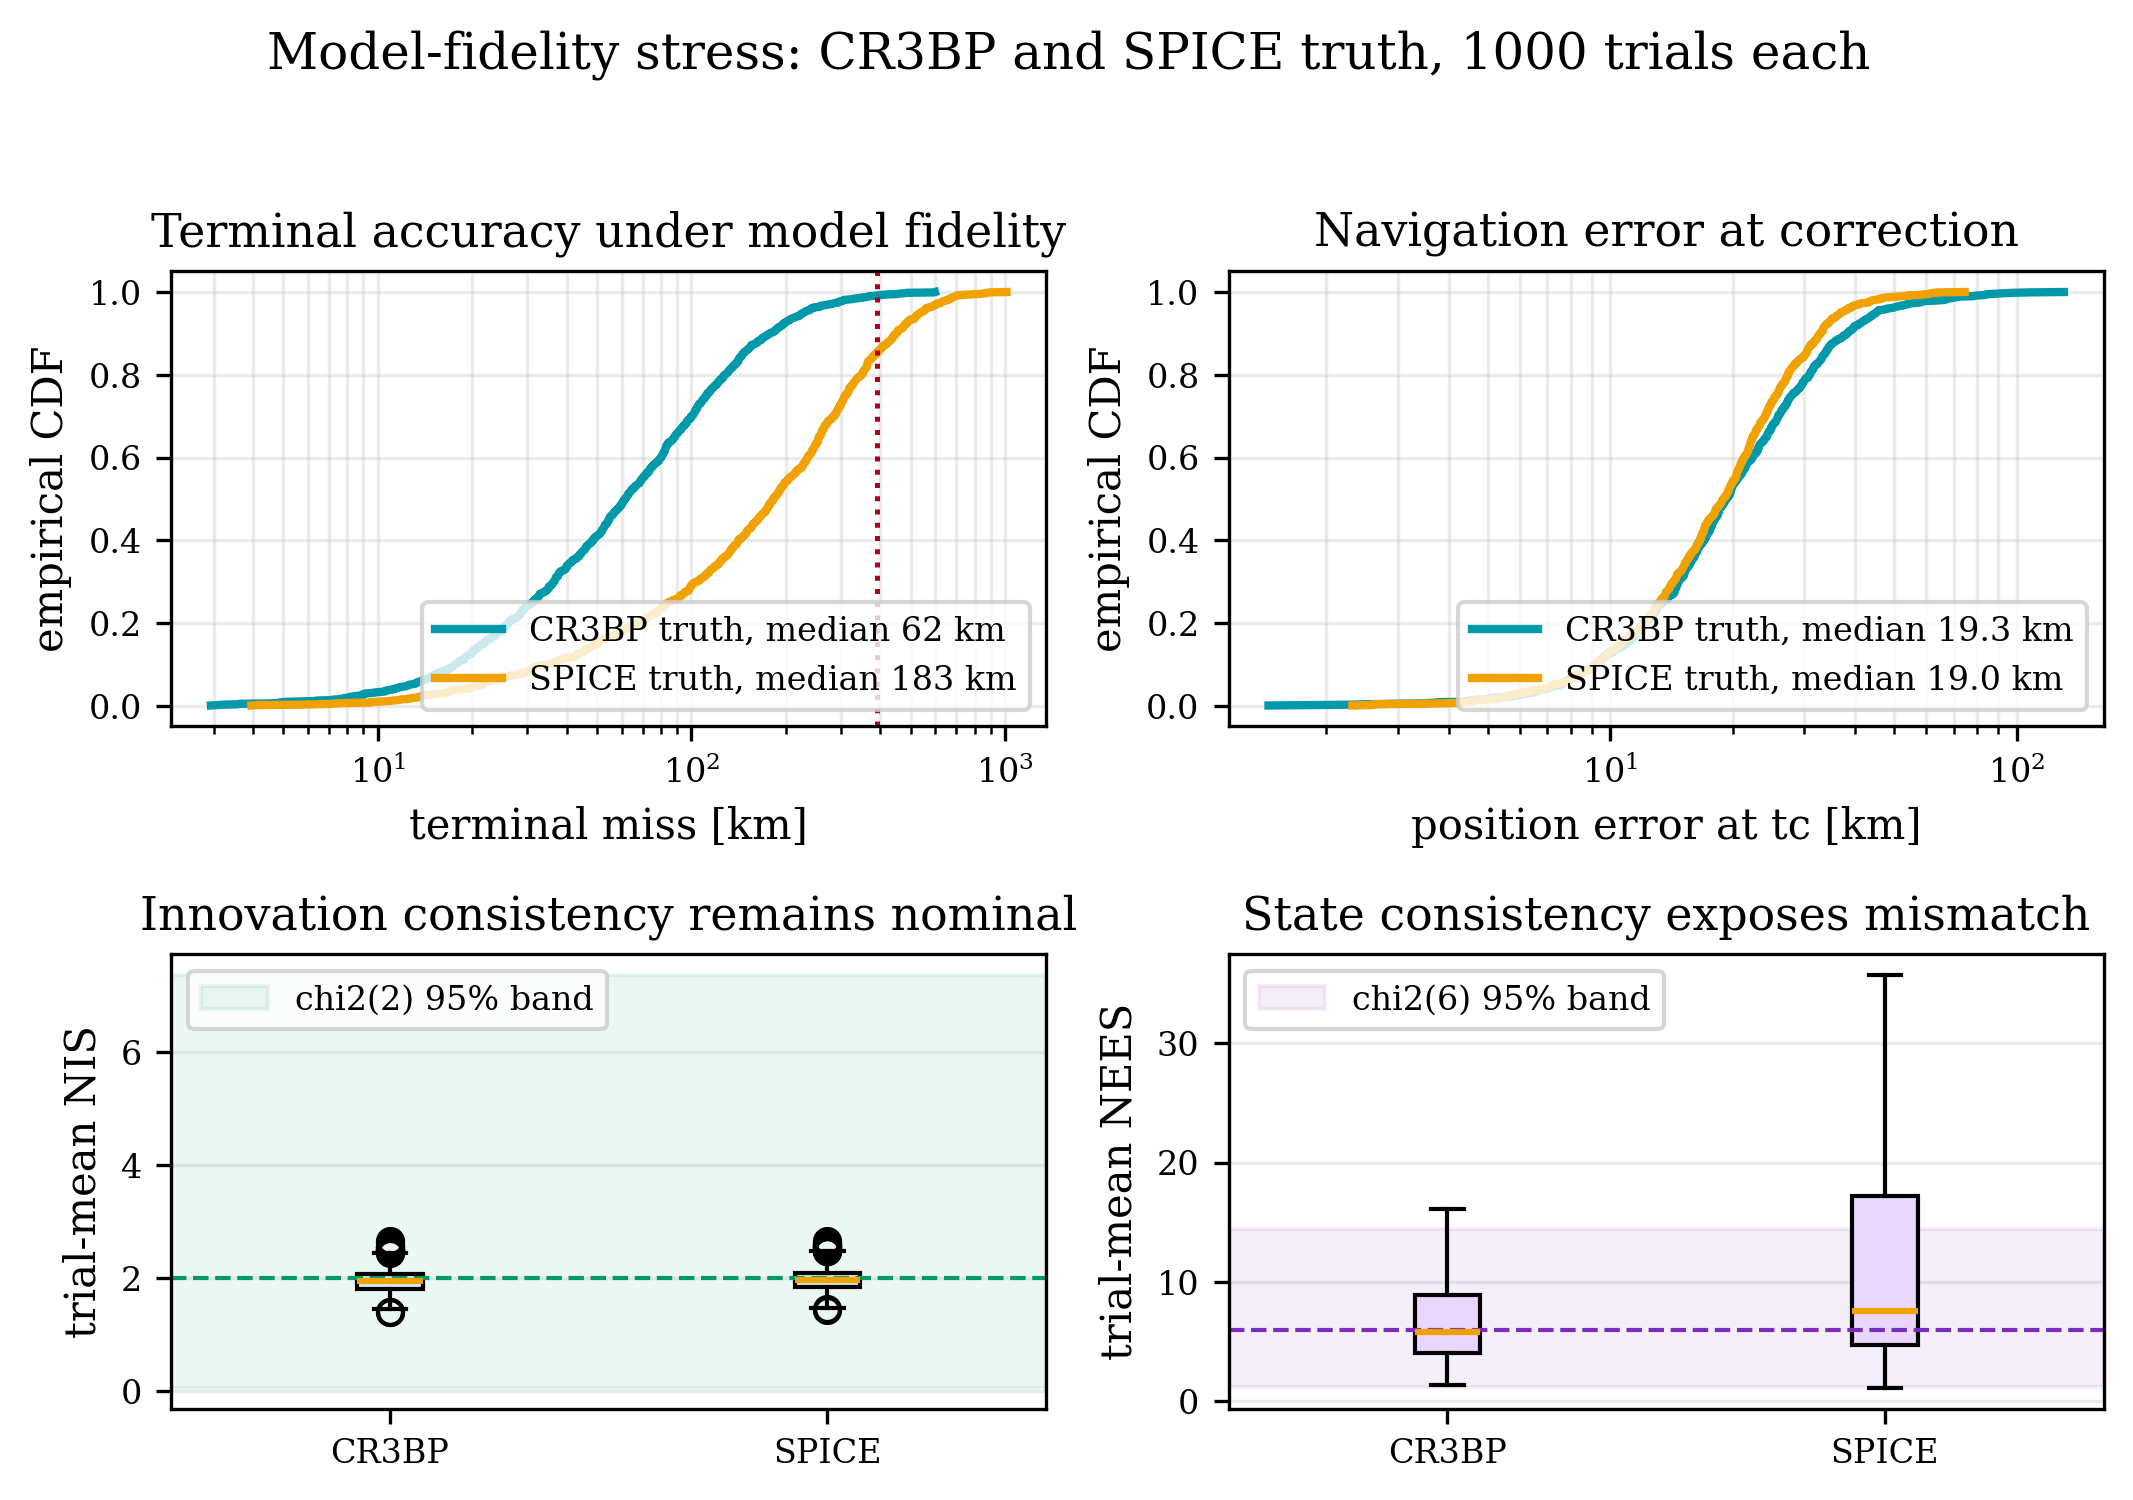
\includegraphics[width=0.9\linewidth]{figures/model_fidelity_summary.png}
\caption{Model-fidelity stress summary for $1000$-trial CR3BP and SPICE point-mass truth cases.  CR3BP errors are converted to kilometres.  NIS remains nominal while NEES and terminal miss reveal the effect of higher-fidelity truth.}
\label{fig:S-model-fidelity}
\end{figure}

\section{Synthetic and Catalog-Backed Landmark Configurations}
\label{sec:S-landmarks}
The L1 and L2 landmark sweeps each run three configurations on identical seeds at $n=1000$ trials per configuration: Moon-center only, landmark-only with the Moon-center disabled, and Moon-plus-landmarks.  Median terminal miss drops from $61.6$~km (Moon-only) to $26.2$~km (landmarks only, L1) and $23.5$~km (Moon+landmarks, L1).  The L2 catalog-backed numbers (Tycho, Copernicus, Aristarchus, Plato, Kepler, Grimaldi) are within $6\%$ of the L1 numbers across all three configurations, confirming that the gain comes from spatial diversity of the bearing rays rather than the symmetric placement of the L1 layout.

\begin{table}[h]
\centering
\caption{L1 (synthetic six-axis) and L2 (catalog six-crater) landmark configurations, $n=1000$ trials per cell, identical seeds across cells.  Pooled NIS is computed over Moon-center plus accepted landmark updates.}
\label{tab:S-landmarks}
\footnotesize
\begin{tabular}{@{}lccccc@{}}
\toprule
Configuration & miss med [km] & miss p95 [km] & pos err [km] & NEES med. & NIS pooled \\
\midrule
\multicolumn{6}{@{}l}{\emph{L1 synthetic six-axis layout}} \\
moon\_only            & 61.64 & 228.27 & 19.32 & 5.78 & 1.94 \\
landmarks\_only       & 26.17 &  72.09 &  7.66 & 4.60 & 1.98 \\
moon $+$ landmarks    & 23.51 &  69.95 &  7.15 & 4.69 & 1.98 \\
\midrule
\multicolumn{6}{@{}l}{\emph{L2 catalog six-crater layout (Tycho/Copernicus/Aristarchus/Plato/Kepler/Grimaldi)}} \\
moon\_only            & 61.64 & 228.27 & 19.32 & 5.78 & 1.94 \\
landmarks\_only       & 26.94 &  73.90 &  7.82 & 4.59 & 1.98 \\
moon $+$ landmarks    & 25.07 &  72.51 &  7.37 & 4.73 & 1.98 \\
\bottomrule
\end{tabular}
\end{table}

\section{Fault and Timing Sensitivity}
Table~\ref{tab:S-vv} summarizes representative diagnostic cases.  The qualitative result is that estimate-tracking and truth-tracking are nearly identical in the nominal case (active pointing itself introduces no significant bias when driven by a good estimate); random dropout and pixel outlier scenarios remain stable in the tested settings; a one-step measurement delay fails as in Section~\ref{sec:S-delay}.

\begin{table}[h]
\centering
\caption{Verification and stress-testing cases on the active-tracking pipeline.}
\label{tab:S-vv}
\footnotesize
\begin{tabular}{@{}lccc@{}}
\toprule
Case & vis.\ fraction & NIS med. & terminal miss [LU] \\
\midrule
Nominal estimate-tracking & 0.997 & 1.715 & $\sim 10^{-4}$ \\
Truth-tracking            & 0.997 & 1.713 & $\sim 10^{-4}$ \\
Dropout                   & 0.960 & 1.792 & $5.26\times10^{-5}$ \\
Pixel outliers            & 1.000 & 1.716 & $7.32\times10^{-5}$ \\
One-step delay            & 0.977 & 1.718 & $2.96\times10^{-3}$ \\
\bottomrule
\end{tabular}
\end{table}

\section{Compute Budget for Production Drivers}
\label{sec:S-compute}
Reviewer-grade reproducibility requires realistic compute expectations.  Table~\ref{tab:S-compute} reports approximate end-to-end wall times for the major production drivers on an eight-core consumer machine.  Per-trial compute is dominated by adaptive-tolerance state-and-STM propagation; the IEKF/EKF updates are sub-millisecond after process-pool startup is amortized.  Full paper-results regeneration is under three hours wall, exclusive of the SPICE-point-mass-truth comparison ($\sim 30$~s/trial single-process), which adds roughly thirty minutes more.

\begin{table*}[h]
\centering
\caption{Approximate wall-clock cost of regenerating the production data backing each main-paper or supplemental table/figure on an eight-core machine.}
\label{tab:S-compute}
\footnotesize
\begin{tabular}{@{}llrr@{}}
\toprule
driver & output dir & cells $\times n$ & wall \\
\midrule
\texttt{06\_monte\_carlo.py}                                & \texttt{phase\_d\_production/}              & $1\!\times\!1000$  & $\sim$30~m \\
\texttt{06f\_compare\_truth\_modes.py}                       & \texttt{phase\_d\_production\_spice/}       & $1\!\times\!1000$  & $\sim$8~h \\
\texttt{06k\_p0\_sensitivity.py}                             & \texttt{phase\_e\_P0/}                       & $5\!\times\!1000$  & $\sim$1~h \\
\texttt{06l\_multi\_revolution.py}                           & \texttt{phase\_e\_multi\_rev/}               & $3\!\times\!100$   & $\sim$30~m \\
\texttt{06m\_parallax\_vs\_range.py}                         & \texttt{phase\_e\_parallax/}                 & $\sim$8000 pts     & $\sim$25~m \\
\texttt{06n\_landmarks.py} (L1, L2)                          & \texttt{phase\_e\_landmarks/}, \texttt{phase\_e\_landmarks\_catalog/} & $3\!\times\!1000$ each & $\sim$25~m each \\
\texttt{06p\_measurement\_delay.py}                          & \texttt{phase\_e\_delay/}                    & $7\!\times\!1000$  & $\sim$50~m \\
\texttt{06q\_attitude\_noise\_sweep.py}                      & \texttt{phase\_e\_attitude\_noise/}          & $7\!\times\!1000$  & $\sim$30~m \\
\texttt{06r\_landmarks\_under\_pointing\_degradation.py}     & \texttt{phase\_f\_landmarks\_pointing/}      & $15\!\times\!1000$ & $\sim$3~m \\
\texttt{06s\_estimator\_ablation.py}                         & \texttt{phase\_g\_estimator\_ablation/}      & $3\!\times\!1000$  & $\sim$5~m \\
\texttt{06t\_success\_ecdf\_central.py}                      & \texttt{phase\_h\_central\_ecdf/}            & post-hoc            & $<$1~s \\
\bottomrule
\end{tabular}
\end{table*}

\section{Modeling Assumptions and Limitations}
\label{sec:S-assumptions}
Table~\ref{tab:S-assumptions} consolidates the modeling assumptions across the paper, indicating for each whether the assumption was stress-tested and where the test appears.

\begin{table*}[h]
\centering
\caption{Modeling assumptions, stress-test status, and what remains out of scope.}
\label{tab:S-assumptions}
\footnotesize
\begin{tabular}{@{}p{0.18\textwidth}p{0.32\textwidth}p{0.22\textwidth}p{0.24\textwidth}@{}}
\toprule
Assumption & Baseline & Stress-tested? & Future work \\
\midrule
Dynamics  & CR3BP estimator; CR3BP or SPICE point-mass truth & Yes: SPICE point-mass truth (\S\ref{sec:S-delay}) & Higher-order non-spherical gravity, SRP \\
Measurement & Ideal body-center pinhole bearing & Partially: pixel noise, dropout, outliers & Limb fitting, photometric bias, false matches \\
Active pointing & Ideal estimate-driven pointing & Yes: bias, lag, attitude-noise sweeps (main Tab.~9; \S\ref{sec:S-attitude}) & Slew limits, actuator dynamics, closed-loop attitude estimation \\
Initial covariance & $\vect{P}_0$ fixed at the value in main Sec.~3.7 & Yes: $\vect{P}_0$ scaling \S\ref{sec:S-attitude} & Adaptive initialization \\
Time tagging & Ideal synchronized measurements & Yes: delay sweep \S\ref{sec:S-delay} & Continuous timing bias, jitter, on-board time-tag estimation \\
Landmarks & L1 (six synthetic) and L2 (six catalog) with known identity & Yes: \S\ref{sec:S-landmarks} and main \S5.4 & L3: image-based detection, catalog association, false-match rejection \\
\bottomrule
\end{tabular}
\end{table*}

\end{document}
